\documentclass[11pt]{article}
\usepackage[margin=30mm]{geometry}
\usepackage[comma]{natbib}
\usepackage{todonotes}
\usepackage[toc,page]{appendix}
\usepackage{pdfpages}
\usepackage{graphicx}
\usepackage{url}

\bibliographystyle{agsm}

\usepackage{listings}
\usepackage{color}
\definecolor{dkgreen}{rgb}{0,0.6,0}
\definecolor{gray}{rgb}{0.5,0.5,0.5}
\definecolor{mauve}{rgb}{0.58,0,0.82}

\lstset{frame=tb,
  language=Python,
  aboveskip=3mm,
  belowskip=3mm,
  showstringspaces=false,
  columns=flexible,
  basicstyle={\small\ttfamily},
  numbers=none,
  numberstyle=\tiny\color{gray},
  keywordstyle=\color{blue},
  commentstyle=\color{dkgreen},
  stringstyle=\color{mauve},
  breaklines=true,
  breakatwhitespace=true,
  tabsize=3
}

\begin{document}
\title{WEP Attacks and Solutions}
\author{Jack Neilson}
\maketitle

\includepdf{1506801_cover_letter.pdf}
\tableofcontents
\newpage

\section{Non-Technical Report}
\subsection{WEP Overview}
Wired Equivalent Privacy (WEP) is a method of securing over-the-air network traffic. It's used when devices connect to a Wi-Fi access spot to make sure that traffic between an access spot and an end device (such as a laptop or mobile phone) is encrypted, and isn't sent "in the clear" as human-readable, unencrypted text. It is important that traffic is encrypted in this manner, as otherwise an attacker could position themselves between an end device and an access point and read every communication sent between the two devices, capturing sensitive information in the process.

\subsection{WEP Implementation}
At it's core, WEP encryption consists of two components:

\begin{itemize}
\item{An "initialisation vector" (IV). This is a random number that is generated for each message sent over the network. It is used in conjunction with the secret key to generate a stream of pseudo-random bits that are suitable for encryption.} 

\item{A secret key. This is known to both the access point and end device, and is used when encrypting and decrypting traffic.}
\end{itemize}

First, the IV and the secret key are joined together to give the key for the message. This is then put through the RC4 algorithm, which generates a stream of pseudo-random numbers.

\vspace{10px}
\centerline{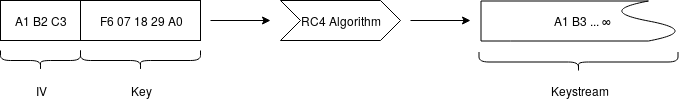
\includegraphics[width=\linewidth]{res/keystream.png}}
\vspace{6px}

A digest (CRC) of the message is then generated to allow to recipient to check for errors.

\vspace{10px}
\centerline{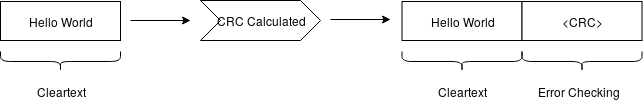
\includegraphics[width=\linewidth]{res/crc.png}}

\newpage
The message and the CRC is then encrypted using the keystream.

\vspace{10px}
\centerline{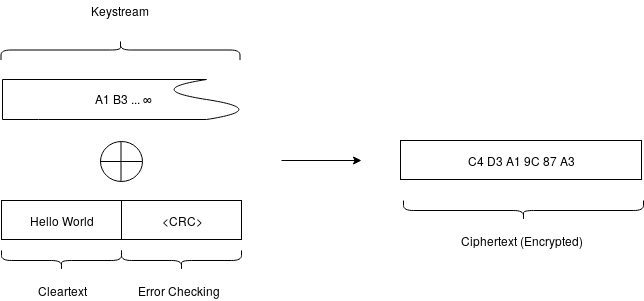
\includegraphics[width=\linewidth]{res/encryption.png}}
\vspace{6px}

Finally, the IV is added so that the recipient can do the entire process in reverse to decrypt to message.

\vspace{10px}
\centerline{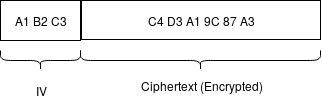
\includegraphics[scale=1.0]{res/header.png}}
\vspace{6px}

\subsection{Weaknesses of WEP}
WEP was superceded by WPA in 2003, and was deprecated due to security concerns in 2004. 

In 2006 a paper was released that showed fundamental flaws in how the WEP standard was designed, allowing attackers to gain access to the key of even the most secure (104-bit) implementations in under 60 seconds\citep{breakingWEP60seconds}. This is particularly damning as the key allows the attacker to decrypt all traffic he or she captures.

\subsection{Business Impact}
The business impact of using WEP with no other mitigations could potentially be very large. Should an attacker come in range of a wi-fi access point they could potentially gather traffic to and from multiple users. If this occurs the massive negative press could potentially bankrupt the business, legal implications notwithstanding. Industry regulators could force the business to close if medical or financial information is disclosed.

\section{Proposed Solution}
\subsection{VPN}

\section{Ethics}
\subsection{Ethical Framework}
\subsection{Professional Standards}

\bibliography{citations}

\end{document}